% Created 2023-05-08 Mon 15:21
% Intended LaTeX compiler: pdflatex
\documentclass[9pt, b5paper]{article}
\usepackage{xeCJK}
\usepackage[T1]{fontenc}
\usepackage{bera}
\usepackage[scaled]{beraserif}
\usepackage[scaled]{berasans}
\usepackage[scaled]{beramono}
\usepackage[cache=false]{minted}
\usepackage{xltxtra}
\usepackage{graphicx}
\usepackage{xcolor}
\usepackage{multirow}
\usepackage{multicol}
\usepackage{float}
\usepackage{textcomp}
\usepackage{algorithm}
\usepackage{algorithmic}
\usepackage{latexsym}
\usepackage{natbib}
\usepackage{geometry}
\geometry{left=1.2cm,right=1.2cm,top=1.5cm,bottom=1.2cm}
\usepackage[xetex,colorlinks=true,CJKbookmarks=true,linkcolor=blue,urlcolor=blue,menucolor=blue]{hyperref}
\newminted{common-lisp}{fontsize=\footnotesize} 
\author{deepwaterooo}
\date{\today}
\title{ET 框架的麻将游戏【斗地主、拖拉机、五子棋等同系列】}
\hypersetup{
 pdfauthor={deepwaterooo},
 pdftitle={ET 框架的麻将游戏【斗地主、拖拉机、五子棋等同系列】},
 pdfkeywords={},
 pdfsubject={},
 pdfcreator={Emacs 28.2 (Org mode 9.5.5)}, 
 pdflang={English}}
\begin{document}

\maketitle
\tableofcontents

本卡五星麻将 基于ET框架 请先能正常运行ET的demo  

\section{介绍:}
\label{sec:org9777ba5}
\begin{itemize}
\item 一款麻将游戏,基于ET框架开发,基本和市面上的,房卡麻将一样,功能基本实现 有匹配模式,房卡模式 录像功能 亲友圈
\item 接入了百度地图sdk,微信登陆,分享和支付
\end{itemize}

\section{运行:}
\label{sec:org64d73aa}
\begin{itemize}
\item 下载项目直接打开Unity工程,进入Init场景。因为服务器到期,无法登录到服务器,可以改为本地服务器来试运行。但因为项目中某些地方可能还是与服务器交互,所以构建出来的ET.exe 无法本地多客户端匹配,但可以使用加入房间模式试玩,以理解源码为主要指标。
\item 注:ETModel.Init.isNetworkBundle 这个字段控制是否 使用本地资源 还是使用网络资源
\item\relax [打好包apk下载](\url{https://gamegather.oss-cn-beijing.aliyuncs.com/kwx.apk})
\item 安卓和IOS工程暂时没有上传,因为涉及到开放平台,见谅!
\end{itemize}

\section{本地启动}
\label{sec:org1e0f300}
\begin{itemize}
\item 服务器端要重新生成一下解决方案
\item 要本地开启Monodb服务器
\item 选择LocalAllServer启动 或者直接打开服务器解决点击启动 效果是一样的

\item 注意事项:  
\begin{itemize}
\item 1.第一次上传的LocalAllServer配置文件 配置不对 熟悉自己改 不熟悉的可以重新下载
\item 2.服务器每次启动都会默认添加一些配置数据 但是如果检测到数据库已经有数据了 就不会添加了 启动失败可以尝试清空本地数据库
\end{itemize}
\end{itemize}

\begin{center}
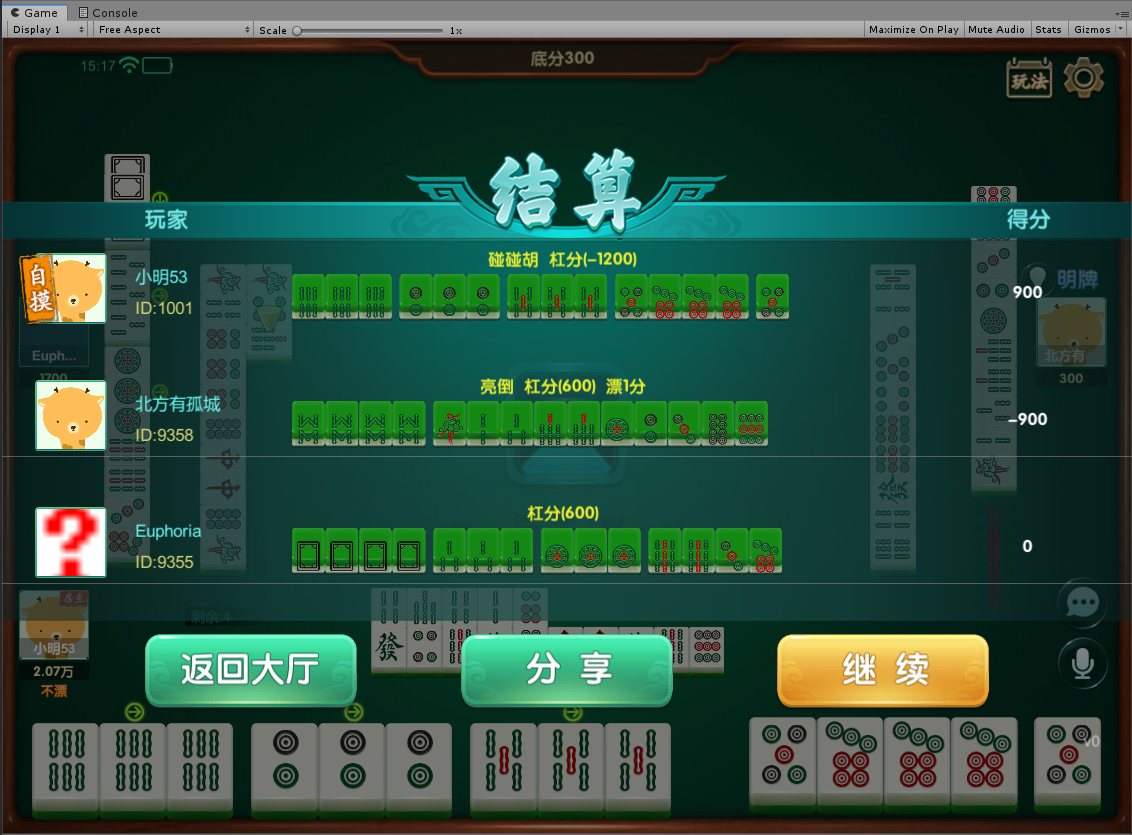
\includegraphics[width=.9\linewidth]{./pic/readme_20230508_151755.png}
\end{center}
\begin{itemize}
\item 以前,这种游戏是想都不用想,超出难度,但现在因为可以使用现有的服务器也可以热更新的 ET 框架,这些想对复杂的游戏都变得简单。
\item 只是好玩儿的游戏,斗地主、跑得快,拖拉机,麻将等,好玩儿的游戏都被 ET 写完了,但小弱弱们写什么游戏练手好呢?【活宝妹就是一定要嫁给亲爱的表哥!!!】
\end{itemize}
\end{document}